\subsection{Template engine}
\subsubsection{Overview}Template engine is a tool for faster and easier building views for our application. 
It allows us to create one big view from little "bricks" - parts of html code. 
The most common situation is when we have page header, menu page, page content and page footer. 
Writing each html file with header and footer can be very boring job. 
Moreover what if at some point of time we decide to change the header? 
We will have to change it's every occurrence in the hundreds of html files (in case of big service).

Template engine is in fact a set of three {\it wtpl} tags: {\it wtpl:parent}, {\it wtpl:include} and {\it wtpl:content}.

\subsubsection{wtpl tags}
\begin{enumerate}
\item {\it $<$wtpl:include name=}{\bf {\em Name}} {\it /$>$} - tag which specifies the place, where the content of corresponding {\it wtpl:content} tag 
(with the same attribute {\bf {\em Name}}) will be inserted. 
\item {\it $<$wtpl:parent path=}{\bf {\em Path}} {\it /$>$} - tag which specifies which template will be filled with {\it wtpl:content} contents. 
It must be the root element of each child template (template, which contains at least one {\it wtpl:content}).
\item {\it $<$wtpl:content name=}{\bf {\em Name}} {\it /$>$} - tag which content will replace corresponding (with the same {\bf {\em Name}} attribute)
 {\it wtpl:include} tag in {\it wtpl:parent} file.
\end{enumerate}
To display the page properly, all the {\it wtpl:include} tags must be substituted with corresponding {\it wtpl:content} tags.

\subsubsection{Control flow}When template expander starts his work and encounters the {\it wtpl:parent} tag - the template engine starts his work. 
The control flow is as follows:
\begin{enumerate}
\item collecting all the insides of {\it wtpl:content} tags
\item loading the file pointed by {\bf Path} attribute in {\it wtpl:parent}
\item fill the possible {\it wtpl:include} slots with corresponding {\it wtpl:content} values
\item if the root element of loaded file is {\it wtpl:parent} expander goes to first step
\end{enumerate} 

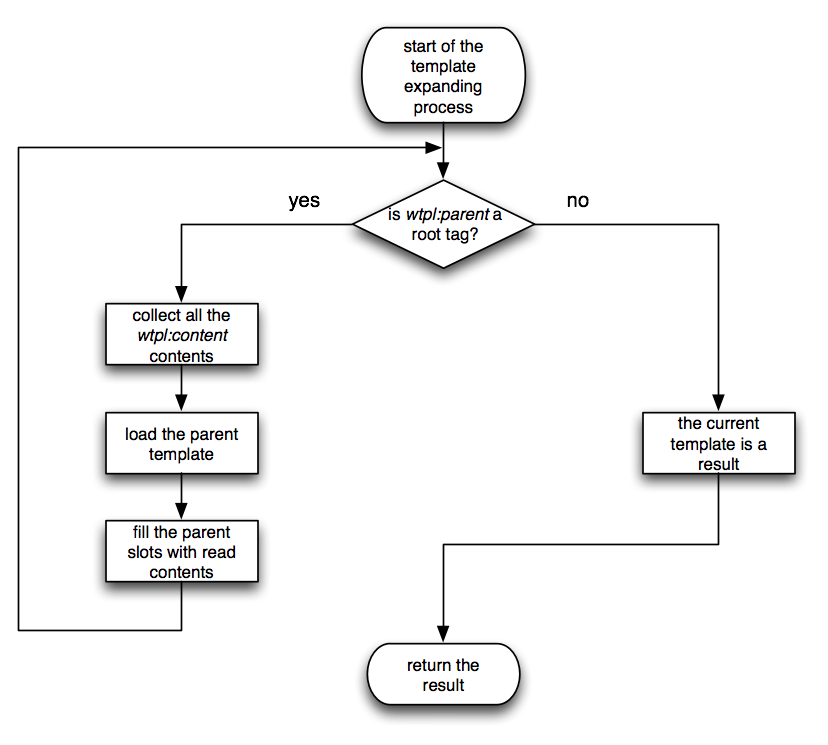
\includegraphics[width=0.95\textwidth]{images/wtpl.jpg}  

\subsubsection{Example}This is an example of nested template html files:

\begin{Verbatim}[numbers=left, frame=single, label=base.html]
<html>
  ...
  <body>
    <wtpl:include name="header"/>
    <wtpl:include name="content"/>
    <wtpl:include name="footer"/>
  </body>
</html>
\end{Verbatim}

\begin{Verbatim}[numbers=left, frame=single, label=half\_filled.html]
<wtpl:parent path="base.html">
  <wtpl:content name="header">
    This is the header of the service
  </wtpl:content>

  <wtpl:include name="menu"/>

  <wtpl:content name="footer">
    This is the footer!
    <img src="footer.jpg"/>
  </wtpl:content>
</wtpl:parent>
\end{Verbatim}

\begin{Verbatim}[numbers=left, frame=single, label=filled.html]
<wtpl:parent path="half_filled.html">
  <wtpl:content name="menu">
    Here we will place our menu
  </wtpl:content>

  <wtpl:content name="content">
    And here will be the content of the page
  </wtpl:content>
</wtpl:parent>
\end{Verbatim}

After expanding, final page ({\it "filled.html"}) will look like that:
\begin{Verbatim}[numbers=left]
<html>
  ...
  <body>
    This is the header of the service
    Here we will place our menu
    And here will be the content of the page
    This is the footer!
    <img src="footer.jpg"/>
  </body>
</html>
\end{Verbatim}

\subsubsection{wpart\_gen} {\it wpart\_gen} module has been created beacuse of the need for building HTML code efficiently inside of the Erlang modules.
The idea was to remove all the HTML tags to the separate files, with extension {\it .tpl}, and to load and fill them in controller.

The usage of the {\it wpart\_gen} module is very simple. 
At the beginning we should load our HTML snippets into the memory in order to access them as fast as we only can.
It could be done by running:
\begin{verbatim}
wpart_gen:load_tpl(Namespace, Name, Path).
\end{verbatim}
This call will load the file from {\it Path} and place it in the memory under the key {\it \{Namespace, Name\}}. 
Namespaces has been implemented because some names are very common, like {\it li} - so we want to recognize them in our controller.
Loading should be performed only once - during the start of our system.

The templates snippets are the normal HTML files, but have several {\it marked} places, where we want to inject our content. 
There are two ways for specifying the templates:
\begin{description}
\item[named slots]- they are used when we do not want to remember the exact order and number of the parameters. 
The slots are specified by their names. 
In case when developer did not pass all names during the template filling, the unfilled slots will be replaced with empty strings.
The syntax is as follows:
\begin{verbatim}
...
<!-- HTMLCode -->
<% name_of_the_slot %>
<!-- HTMLCode -->
...
\end{verbatim}

\item[anonymous slots]- has been implemented in order to achieve better efficency.
We must remember the exact number of the slots and their order:
\begin{verbatim}
...
<!-- HTMLCode -->
<% slot %>
<!-- HTMLCode -->
...
\end{verbatim}
\end{description}

When we have the snippets prepared and loaded, they are ready to use. 
In order to get the snippet we should call
\begin{verbatim}
wpart_gen:tpl_get(Namespace, Name)
\end{verbatim}
Then, to fill the template with our values, we should call
\begin{verbatim}
wpart_gen:build_hml(Tpl, Values)
\end{verbatim}
where {\it Tpl} is a template loaded in previous call and {\it Values} is a list of our specific values.
{\it Values} list format depends on the type of the slots we used:
\begin{description}
\item[named slots]- we should pass the list of tagged tuples:
\begin{verbatim}
[{"name_of_the_slot", Value} | ...]
\end{verbatim}
The slot with the specified name will be substituted with the corresponding {\it Value} which is a string. 
We do not have to pass all the values - the unfilled slots will remain empty.

\item[anonymous slots]- we should pass a list of values:
\begin{verbatim}
[Value | ...]
\end{verbatim}
Length of that list must be the same as the number of the slots defined in the snippet. 
If the lengths differ, the {\it erlang:error} function will be called.
Moreover, the order is important here - we have to build the list of values in the correct sequence.
\end{description}

The properly prepared HTML code could be returned as the value of the \#xmlText record from the handle\_call function.
